\section{Case Study}\label{sec:case-study}
The proposed architecture is mainly based on the approaches presented by \cite{fraunholz2018industrial} and complemented with industrial intrusion detection models proposed in \cite{sayegh2019ids}.

The architecture follows a hierarchical industrial network design based on IT/OT segmentation and the deployment of an Intrusion Prevention System (IPS) to mitigate Denial of Service (DoS) attacks targeting Programmable Logic Controllers (PLCs) and industrial switches.

The proposed solution incorporates:
\begin{itemize}
    \item Network segmentation using VLANs,
    \item Separation between IT and OT environments,
    \item Inline IPS inspection,
    \item Monitoring of industrial protocols,
    \item Protection of PLC communication channels.
\end{itemize}

According to Fraunholz et al. \cite{fraunholz2018industrial}, industrial IPS architectures should provide reactive protection mechanisms capable of identifying malicious traffic patterns and preventing attacks before they impact industrial devices.

Additionally, Ahmed et al. \cite{ahmed2019survey}, recommend the implementation of Purdue-based segmentation models to isolate operational technology (OT) networks from corporate infrastructures.

The proposed architecture aims to:
\begin{itemize}
    \item Protect PLCs against DoS attacks,
    \item Improve industrial network availability,
    \item Detect anomalous industrial traffic,
    \item Reduce propagation of attacks within OT environments,
    \item Maintain stable communication between SCADA systems and PLCs.
\end{itemize}

\subsection{Network Architecture}
The network architecture follows a layered industrial control system (ICS) design inspired by the Purdue Enterprise Reference Architecture and the IPS deployment proposed by Fraunholz et al. \cite{fraunholz2018industrial}.

The architecture separates the corporate network from the operational network using firewalls, industrial switches, VLAN segmentation, and an inline Intrusion Prevention System (IPS).

The IPS is strategically deployed between the SCADA layer and the PLC network in order to inspect traffic in real time and mitigate potential flooding attacks targeting industrial devices.

The proposed architecture includes the following components:

\begin{table}[htbp]
\caption{Components of the Proposed Industrial Architecture} 
\centering
\scriptsize
\resizebox{\columnwidth}{!}{%
\begin{tabular}{l c c}
\toprule
\textbf{Component} & \textbf{Function} & \textbf{Reference} \\
\midrule
PLC & Industrial process control & \cite{fraunholz2018industrial} \\
SCADA/HMI & Monitoring and supervision & \cite{fraunholz2018industrial} \\
Industrial Switch & VLAN segmentation and traffic control & \cite{sayegh2019ids} \\
Firewall & IT/OT network separation & \cite{ahmed2019survey} \\
IPS (Suricata/Snort) & Attack detection and mitigation & \cite{fraunholz2018industrial} \\
Monitoring Station & Traffic analysis and packet capture & \cite{sayegh2019ids} \\
Attacker Machine & DoS attack generation & Experimental environment \\
\bottomrule
\end{tabular}%
}
\end{table}


The industrial switch is responsible for managing VLAN segmentation and isolating traffic between the SCADA network and PLC devices. According to Sayegh et al. \cite{sayegh2019ids}, segmentation mechanisms improve the security posture of industrial Ethernet networks by reducing unnecessary broadcast traffic and limiting attack propagation.

The IPS performs Deep Packet Inspection (DPI) on industrial protocols such as Modbus/TCP and Ethernet/IP. This allows the detection of abnormal traffic patterns associated with DoS attacks.

The architecture also incorporates a Demilitarized Zone (DMZ) between the enterprise network and the industrial network to provide an additional security layer, as recommended in \cite{ahmed2019survey}.

\subsection{Topology}
The proposed topology follows a hierarchical Industrial Control System (ICS) architecture inspired by the Purdue Enterprise Reference Model and the distributed intrusion detection approach proposed by Mansfield et al. \cite{mansfield2020threeTier}.

The architecture separates the corporate network from the operational technology (OT) environment through the use of firewalls, industrial switches, and VLAN segmentation. An inline Intrusion Prevention System (IPS) is deployed between the SCADA layer and the PLC network to monitor and mitigate malicious traffic in real time.

The proposed topology is illustrated in Figure~\ref{fig:industrial_topology}.

\begin{figure}[H]
    \centering
    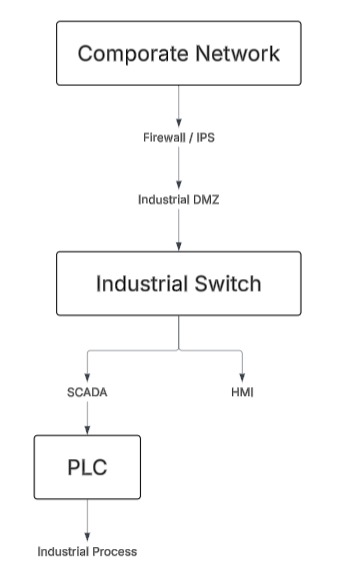
\includegraphics[width=0.3\textwidth]{network_topology.jpeg}
    \caption{Proposed industrial network topology}
    \label{fig:industrial_topology}
\end{figure}

According to Fraunholz et al. \cite{fraunholz2018industrial}, network segmentation and the implementation of a DMZ reduce the propagation of attacks within industrial environments and improve the monitoring capabilities of security systems.

The industrial switch is responsible for managing traffic isolation between VLANs and prioritizing industrial communications. Sayegh et al. \cite{sayegh2019ids}, indicate that traffic segmentation improves the resilience of industrial Ethernet networks against denial-of-service attacks.

The proposed VLAN segmentation is presented in Table~\ref{tab:vlan_segmentation}.

\begin{table}[htbp]
\caption{Proposed VLAN Segmentation} 
\scriptsize 
\begin{tabular}{l c c c} 
\toprule
\textbf{VLAN} & \textbf{Purpose} & \textbf{Reference} \\
\midrule
VLAN 10 & Corporate network & Purdue Model \\
VLAN 20 & SCADA/HMI communication & \cite{ahmed2019survey} \\
VLAN 30 & PLC network & \cite{fraunholz2018industrial} \\
VLAN 99 & Network management & Industrial segmentation practice \\
\bottomrule
\end{tabular}
\label{tab:vlan_segmentation}
\end{table}

\subsection{IPS Configuration}

The Intrusion Prevention System (IPS) configuration is based on the reactive protection architecture proposed by Fraunholz et al. \cite{fraunholz2018industrial}. The IPS is deployed in inline mode to inspect industrial traffic before it reaches PLC devices.

The IPS performs Deep Packet Inspection (DPI) on industrial communication protocols such as Modbus/TCP and Ethernet/IP. According to Sayegh et al. \cite{sayegh2019ids}, protocol-aware traffic inspection improves the detection accuracy of attacks targeting industrial control systems.

The proposed IPS configuration parameters are presented in Table~\ref{tab:ips_configuration}.

\begin{table}[htbp]
\caption{IPS Configuration Parameters} 
\centering
\scriptsize
\resizebox{\columnwidth}{!}{%
\begin{tabular}{l c c}
\toprule
\textbf{Parameter} & \textbf{Configuration} & \textbf{Reference} \\
\midrule
IPS Tool & Suricata & \cite{fraunholz2018industrial} \\
Deployment Mode & Inline & \cite{fraunholz2018industrial} \\
Protected Protocol & Modbus/TCP & \cite{sayegh2019ids} \\
Detection Method & Signature-based & \cite{fraunholz2018industrial} \\
Packet Inspection & Deep Packet Inspection (DPI) & \cite{sayegh2019ids} \\
Logging & Enabled & Security monitoring practice \\
Automatic Blocking & Enabled & Reactive protection approach \\
\bottomrule
\end{tabular}%
}
\label{tab:ips_configuration}
\end{table}


The IPS uses custom detection rules to identify traffic flooding attacks directed to the PLC communication port (TCP port 502).

An example of a Suricata detection rule is shown below:

\begin{verbatim}
alert tcp any any -> 192.168.1.10 502
(msg:"Possible Modbus TCP Flood";
flow:to_server;
threshold:type both, track by_src,
count 50, seconds 1;
sid:100001;)
\end{verbatim}

The rule detects excessive TCP requests directed to the Modbus/TCP service and generates alerts when abnormal traffic thresholds are exceeded.

According to Fraunholz et al. \cite{fraunholz2018industrial}, inline IPS deployment allows real-time mitigation actions such as:
\begin{itemize}
    \item automatic packet filtering,
    \item malicious IP blocking,
    \item rate limiting,
    \item abnormal traffic isolation.
\end{itemize}

\subsection{Attack Scenarios}

The attack scenarios were designed based on methodologies commonly used in Industrial Control System (ICS) security research to evaluate the effectiveness of intrusion prevention systems against Denial of Service (DoS) attacks.

According to Fraunholz et al. \cite{fraunholz2018industrial}, PLCs are particularly vulnerable to flooding attacks due to their limited computational resources and strict real-time communication requirements.

The experimental environment considers multiple attack scenarios targeting industrial communication services such as Modbus/TCP.

\subsubsection{Scenery 1 -- TCP SYN Flood}

The first attack scenario consists of a TCP SYN Flood directed toward the PLC Modbus/TCP service operating on port 502.

The objective of this attack is to saturate the communication resources of the PLC by generating a massive number of incomplete TCP connection requests.

The attack is generated using the \texttt{hping3} tool:

\begin{verbatim}
hping3 -S --flood -V -p 502 192.168.1.10
\end{verbatim}

According to Ahmed et al. \cite{ahmed2019survey}, SYN Flood attacks can significantly degrade the availability of industrial services and interrupt SCADA communications.

\subsubsection{Scenery 2 -- Modbus/TCP Flood}

This scenario focuses on flooding the PLC with excessive Modbus/TCP requests.

The attack simulates malicious traffic directed toward industrial communication protocols in order to overload the PLC processing capabilities.

According to Sayegh et al. \cite{sayegh2019ids}, abnormal traffic patterns in industrial Ethernet protocols can negatively affect:
\begin{itemize}
    \item PLC response time,
    \item SCADA communication stability,
    \item network throughput,
    \item industrial process availability.
\end{itemize}

The attack traffic may be generated using tools such as:
\begin{itemize}
    \item Scapy,
    \item Modbus testing utilities,
    \item custom packet generators.
\end{itemize}

\subsubsection{Scenery 3 -- ICMP Flood}

The third attack scenario consists of an ICMP Flood attack targeting the industrial network.

The objective is to consume network bandwidth and increase communication latency between SCADA systems and PLC devices.

The attack can be generated using the following command:

\begin{verbatim}
ping -f 192.168.1.10
\end{verbatim}

According to Fraunholz et al. \cite{fraunholz2018industrial}, excessive ICMP traffic may affect the stability of industrial Ethernet communications and reduce system availability.

The evaluation variables used during the experiments are presented in Table~\ref{tab:evaluation_variables}.

\begin{table}[htbp]
\caption{Evaluation Variables for Attack Scenarios} 
\centering
\scriptsize
\resizebox{\columnwidth}{!}{%
\begin{tabular}{l c c}
\toprule
\textbf{Variable} & \textbf{Description} & \textbf{Reference} \\
\midrule
Packet Loss & Lost packets during attacks & \cite{fraunholz2018industrial} \\
Latency & Communication delay & \cite{sayegh2019ids} \\
Detection Rate & IPS attack detection accuracy & \cite{mansfield2020threeTier} \\
CPU Usage & PLC resource consumption & \cite{ahmed2019survey} \\
Network Throughput & Network traffic performance & ICS performance metrics \\
Availability & Operational continuity of PLC services & \cite{fraunholz2018industrial} \\
\bottomrule
\end{tabular}%
}
\label{tab:evaluation_variables}
\end{table}


\subsection{Experimental Procedure}
The experimental procedure follows the evaluation methodologies proposed by Fraunholz et al. \cite{fraunholz2018industrial} and Mansfield et al. \cite{mansfield2020threeTier} for industrial intrusion detection and prevention systems.

The experiments are conducted in a controlled industrial network environment composed of:
\begin{itemize}
    \item PLC devices,
    \item SCADA/HMI systems,
    \item industrial switches,
    \item an inline IPS,
    \item an attacker workstation,
    \item monitoring and traffic analysis tools.
\end{itemize}

The experimental methodology is divided into five phases.

\subsubsection{Phase 1 -- Environment Setup}

The first phase consists of configuring the industrial environment and communication infrastructure.

The following components are deployed:
\begin{itemize}
    \item PLC simulation or physical PLC,
    \item SCADA monitoring software,
    \item industrial Ethernet switch,
    \item Suricata IPS,
    \item Wireshark traffic analyzer,
    \item Kali Linux attacker machine.
\end{itemize}

According to Ahmed et al. \cite{ahmed2019survey}, realistic industrial testbeds are essential for evaluating the effectiveness of security mechanisms in ICS environments.

\subsubsection{Phase 2 -- Baseline Traffic Capture}

Normal industrial communication traffic is captured before launching attacks.

The objective of this phase is to establish baseline operational behavior for:
\begin{itemize}
    \item Modbus/TCP communication,
    \item SCADA--PLC interaction,
    \item network latency,
    \item packet delivery rate.
\end{itemize}

Traffic analysis is performed using Wireshark and IPS monitoring logs.

\subsubsection{Phase 3 -- Attack Execution}

During this phase, the attack scenarios described in Section 4.4 are executed against the industrial network.

The generated attacks include:
\begin{itemize}
    \item TCP SYN Flood,
    \item ICMP Flood,
    \item Modbus/TCP Flood.
\end{itemize}

The attacks are generated from the attacker workstation connected to the OT network.

\subsubsection{Phase 4 -- IPS Activation}

The IPS is activated in inline mode with predefined detection and mitigation rules.

According to Fraunholz et al. \cite{fraunholz2018industrial}, reactive IPS mechanisms allow real-time mitigation of malicious traffic before it reaches industrial devices.

The IPS performs:
\begin{itemize}
    \item traffic inspection,
    \item malicious packet filtering,
    \item automatic alert generation,
    \item attack blocking.
\end{itemize}

\subsubsection{Phase 5 -- Performance Evaluation}

The final phase evaluates the effectiveness of the proposed architecture based on the collected metrics.

The evaluation focuses on:
\begin{itemize}
    \item IPS detection accuracy,
    \item false positive rate,
    \item reduction of malicious traffic,
    \item PLC availability,
    \item network latency,
    \item industrial communication stability.
\end{itemize}

According to Mansfield et al. \cite{mansfield2020threeTier}, performance analysis is essential to determine whether security mechanisms introduce operational overhead in industrial control environments.
